\documentclass[uplatex,dvipdfmx]{jlreq}

\usepackage{jlreq-deluxe}
\usepackage[uplatex,deluxe]{otf} % UTF
\usepackage[noalphabet]{pxchfon} % otfの後に1回だけ読み込む
\usepackage{stix2} % 欧文＆数式フォント
\usepackage[fleqn,tbtags]{mathtools} % 数式関連
\usepackage{hira-stix} % ヒラギノフォント＆STIX2 フォント代替定義
\usepackage{float}
\usepackage[hyphens]{url} % urlパッケージ
\usepackage[
  colorlinks=false,            
  pdfborder={0 0 0}
]{hyperref}
\Urlmuskip=0mu plus 1mu  

\usepackage{tabularx}
\usepackage{array}
 \usepackage{multirow}
\renewcommand{\tabularxcolumn}[1]{m{#1}} 
\newcolumntype{C}{>{\centering\arraybackslash}X} 
\usepackage{wrapfig}
\usepackage{amsmath} 
\usepackage{mathtools} 

\usepackage{listings}
\usepackage{xcolor} % 色をつける場合

% ソースコードの見た目の設定
\lstset{
  language={C++},
  basicstyle={\ttfamily\small},
  keywordstyle={\color{blue}},
  commentstyle={\color{green!60!black}},
  stringstyle={\color{orange}},
  frame=single,          % 枠線
  breaklines=true,       % 行が長い場合に折り返す
  numbers=left,          % 行番号を左に表示
  numberstyle={\tiny},
  stepnumber=1,
  showstringspaces=false
}

\usepackage{ascmac}

\begin{document}


\title{担当箇所の基本設計・詳細設計書\_ver光同期廃止後}
\author{25G1113　廣岡花　グループ7}
\date{2026年6月22日}
\maketitle

\section{担当箇所の基本設計}
\subsection{機能一覧}
%ここにFBSを分割したもの，表を入れて詳細に説明
図\ref{fig:1-4}に担当箇所である同期制御機能を中心に詳細化したFBS図を示す．また表\ref{tab:1-3}に，各機能の概要と実装上の要点をまとめる．本システムは，1台のPC（Processing）を指揮者UI，1台のMaster Arduinoを制御ハブ，4台のSlave Arduinoを各楽器ノードとして構成し，Processingから受け取った演奏設定をMaster Arduinoが集約して各Slaveへ配信することで，複数ノードの演奏を協調制御する．Processing側では，ユーザーからBPM，オクターブ，演奏順を受け付け，演奏開始後はBPM以外の操作を自動でロックする．また，受信した再生状態に応じてUIロックを解除する．
本システムの通信は，演奏開始時に送信される初回一括設定パケットと，演奏中に送信されるテンポパケットの2段階で構成される．初回一括設定パケットでは，オクターブ，演奏順，BPMを8バイトの情報としてProcessingからMasterへ送信し，演奏中はBPMのみを送る．Master Arduinoは受信したBPMから8分音符1つあたりの実時間間隔を算出し，その周期でI2Cバスへテンポパルスを送信する．Slave Arduinoはこのテンポパルスを受信するたびに内部のパルスカウンタを進め，担当順番に応じた待機パルス数に達した時点で演奏状態へ移行し，MIDI音高データをProcessingへ送信する．Processingは受信したデータをもとに発音処理を行う．演奏中の状態遷移はProcessing側のserialEvent()でSTART，FINISHを受信することで管理され，UI操作の可否もこれに連動して制御される．

\begin{figure}[H]
    \centering
    \makebox[0pt][c]{
    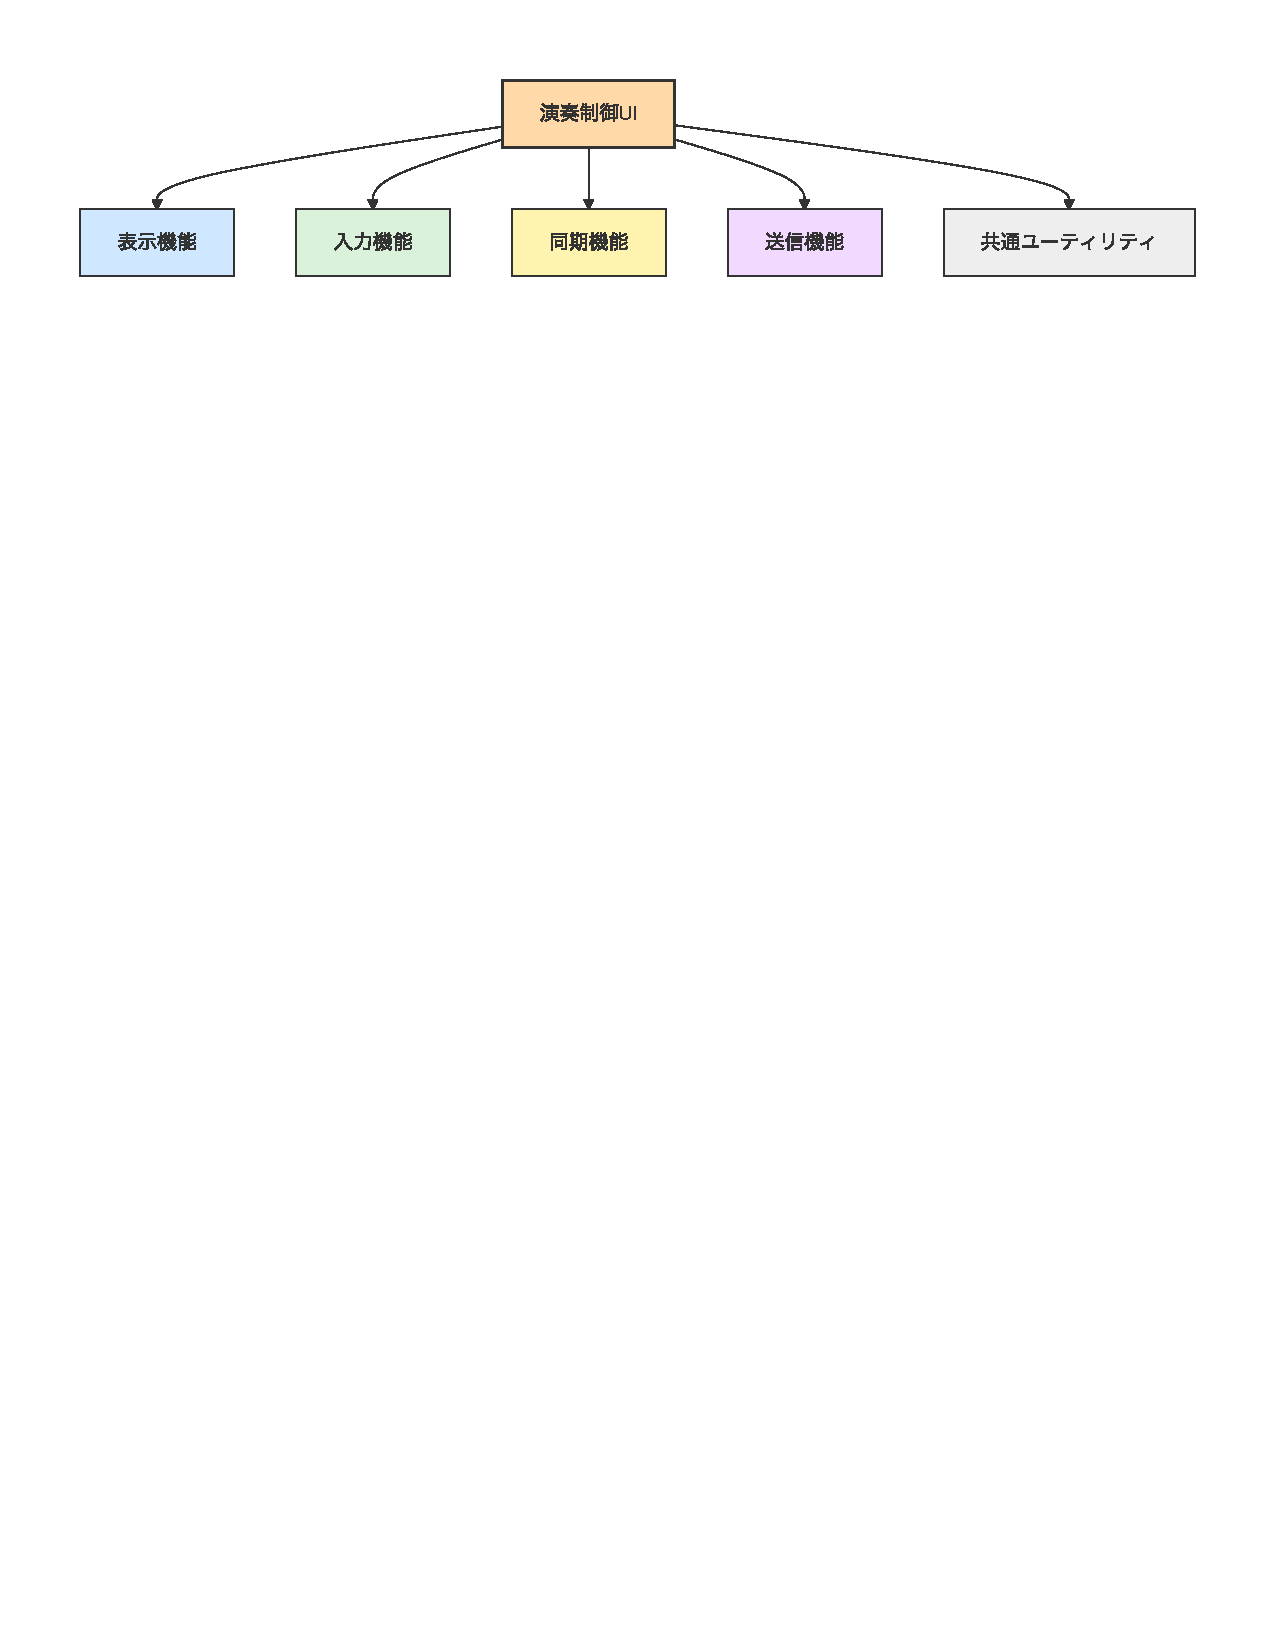
\includegraphics[width=150mm]{fig/FBS.pdf}
    }
    \caption{UI面の同期・表示に着目したFBS}
    \label{fig:1-4}
\end{figure}

\begin{table}[H]
  \centering
  \caption{演奏制御UIの機能一覧}
  \label{tab:1-3}
  \renewcommand{\arraystretch}{1.2}

  \begin{tabularx}{\linewidth}
    {|>{\raggedright\arraybackslash}p{3.0cm}
     |>{\raggedright\arraybackslash}X|}
    \hline
    \textbf{区分} & \textbf{内容} \\ \hline

    \multirow{6}{*}{表示機能}
      & タイトルおよび送信ボタンの描画 \\ \cline{2-2}
      & BPM設定エリアの描画 \\ \cline{2-2}
      & 演奏順番設定エリアの描画 \\ \cline{2-2}
      & 共通オクターブ設定エリアの描画 \\ \cline{2-2}
      & Slave状態ボックスの描画 \\ \cline{2-2}
      & 送信パケットおよび状態情報の表示 \\ \hline

    \multirow{2}{*}{入力機能}
      & ↑／↓キーによるBPM変更，1\UTF{FF5E}3キーによる演奏順登録 \\ \cline{2-2}
      & 設定送信，順番リセット，オクターブ変更ボタンの操作 \\ \hline

    \multirow{3}{*}{同期機能}
      & START／PLAYING受信時のUIロック，FINISH／STOP受信時の解除 \\ \cline{2-2}
      & isPlayingフラグによる操作制御（演奏順・オクターブ変更禁止，BPM変更のみ許可） \\ \cline{2-2}
      & シミュレーションモード時の擬似ロックおよび手動解除 \\ \hline

    \multirow{2}{*}{送信機能}
      & オクターブ・演奏順・BPMを含む初回設定パケットの生成 \\ \cline{2-2}
      & 初回設定送信および演奏中のBPM更新送信 \\ \hline

    \multirow{2}{*}{共通ユーティリティ}
      & ボタン領域のホバー判定 \\ \cline{2-2}
      & 演奏順および選択状態の初期化 \\ \hline

  \end{tabularx}
\end{table}

\newpage

\subsection{具体的な実装内容}
%各分割したシステムごとの具体的な実装内容

\subsubsection{UI設定入力}

\begin{figure}[H]
    \centering
    \makebox[0pt][c]{
    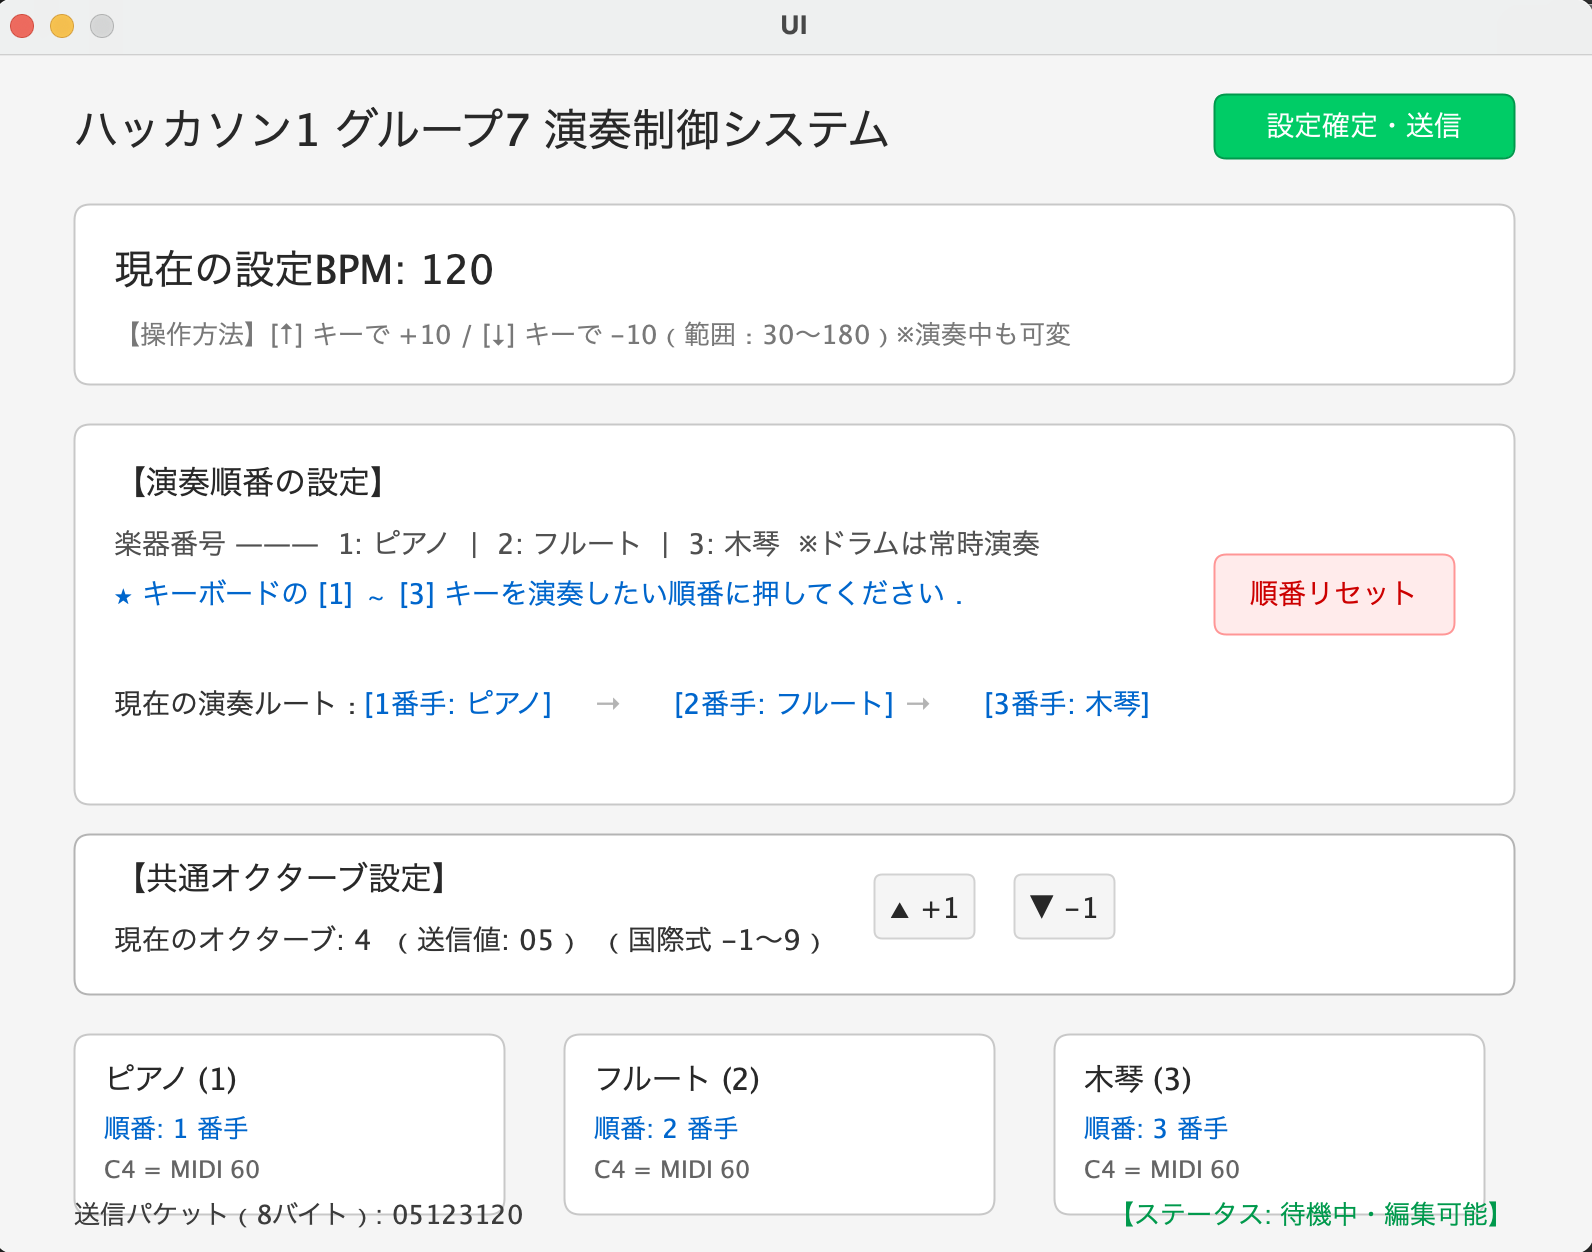
\includegraphics[width=130mm]{fig/UIgamen.png}
    }
    \caption{実際のProcessingのUI画面}
    \label{fig:1-5}
\end{figure}


図\ref{fig:1-5}に本システムの実際のUI画面，表\ref{tab:1-4}にUI画面上の主要な操作要素と，それぞれの操作方法および演奏中の挙動を示す．
本システムのUI画面は，BPM設定エリア，演奏順番設定エリア，共通オクターブ設定エリアの3つの操作領域と，画面右上に配置した設定確定・送信ボタンから構成される．各操作領域は，演奏中であるかどうかを示すフラグ\texttt{isPlaying}の状態に応じて編集可否が切り替わり，ロック中は背景色を淡いグレーに変化させるとともに，該当ボタンを非活性表示にすることで，操作可能な項目を視覚的に明示している．
BPM設定エリアでは，キーボードの[$\uparrow$]キーを押すたびにBPMを$10$加算し，[$\downarrow$]キーを押すたびに$10$減算する．BPMは$30$から$180$の範囲に制限されており，この範囲を超える入力は無視される．BPMのみは演奏中であっても変更を許可しており，テンポを動的に調整できる設計としている．
演奏順番設定エリアでは，楽器番号に対応するキー（[1]：ピアノ，[2]：フルート，[3]：木琴）を押した順に演奏順を確定する．ドラムは演奏開始から常時演奏されるため，演奏順設定の対象から除外している．設定した順番は画面中央に「1番手」「2番手」「3番手」の形式で表示され，未選択の楽器は「未選択」と表示される．また，画面右側に配置した順番リセットボタン（クリック操作）を押すことで，演奏順番の選択状態を初期化できる．演奏中はこの操作領域全体がロックされ，キー入力を受け付けないとともに，リセットボタンの表示も「ロック中」に変化する．
共通オクターブ設定エリアでは，画面下部に配置した[$\blacktriangle$]ボタンおよび[$\blacktriangledown$]ボタンのクリック操作によってオクターブを1ずつ変更する．オクターブは国際式表記で$-1$から$9$の範囲とし，上限・下限を超える操作は無視される．演奏中はオクターブの加減ボタンが非活性表示となり，変更できない状態になる．

\begin{table}[H]
    \centering
    \caption{UI画面における主要操作要素と挙動}
    \label{tab:1-4}
    \small
    \renewcommand{\arraystretch}{1.3}
    \newcolumntype{M}[1]{>{\centering\arraybackslash}m{#1}}
    \newcolumntype{Y}{>{\centering\arraybackslash}X}
    \begin{tabularx}{\textwidth}{|M{3.2cm}|M{4.0cm}|Y|}
        \hline
        \textbf{UI要素} & \textbf{操作方法} & \textbf{演奏中の挙動} \\ \hline

        設定確定・送信ボタン &
        クリックにより設定をパケット化してMaster Arduinoへ送信する &
        常に有効．初回は8バイトの初期パケット，2回目以降はBPM3バイトの差分パケットを送信する
        \\ \hline

        BPM設定 &
        [$\uparrow$]キーで$+10$，[$\downarrow$]キーで$-10$（範囲：$30$〜$180$） &
        演奏中も変更可能
        \\ \hline

        演奏順番設定 &
        [1]〜[3]キーを演奏したい順に押下し，ピアノ・フルート・木琴の演奏順を確定する &
        ロックされ入力を受け付けない
        \\ \hline

        順番リセットボタン &
        クリックにより演奏順番の選択状態を初期化する &
        ボタン表示が「ロック中」に変化し操作不可となる
        \\ \hline

        オクターブ[$\blacktriangle$]ボタン &
        クリックでオクターブを$+1$する（上限$9$） &
        非活性表示となり操作不可となる
        \\ \hline

        オクターブ[$\blacktriangledown$]ボタン &
        クリックでオクターブを$-1$する（下限$-1$） &
        非活性表示となり操作不可となる
        \\ \hline

    \end{tabularx}
\end{table}

\newpage

\subsubsection{Master Arduinoへのシリアル送信処理}

\begin{wrapfigure}{r}{0.45\textwidth}
    \vspace{-2em}
    \centering
    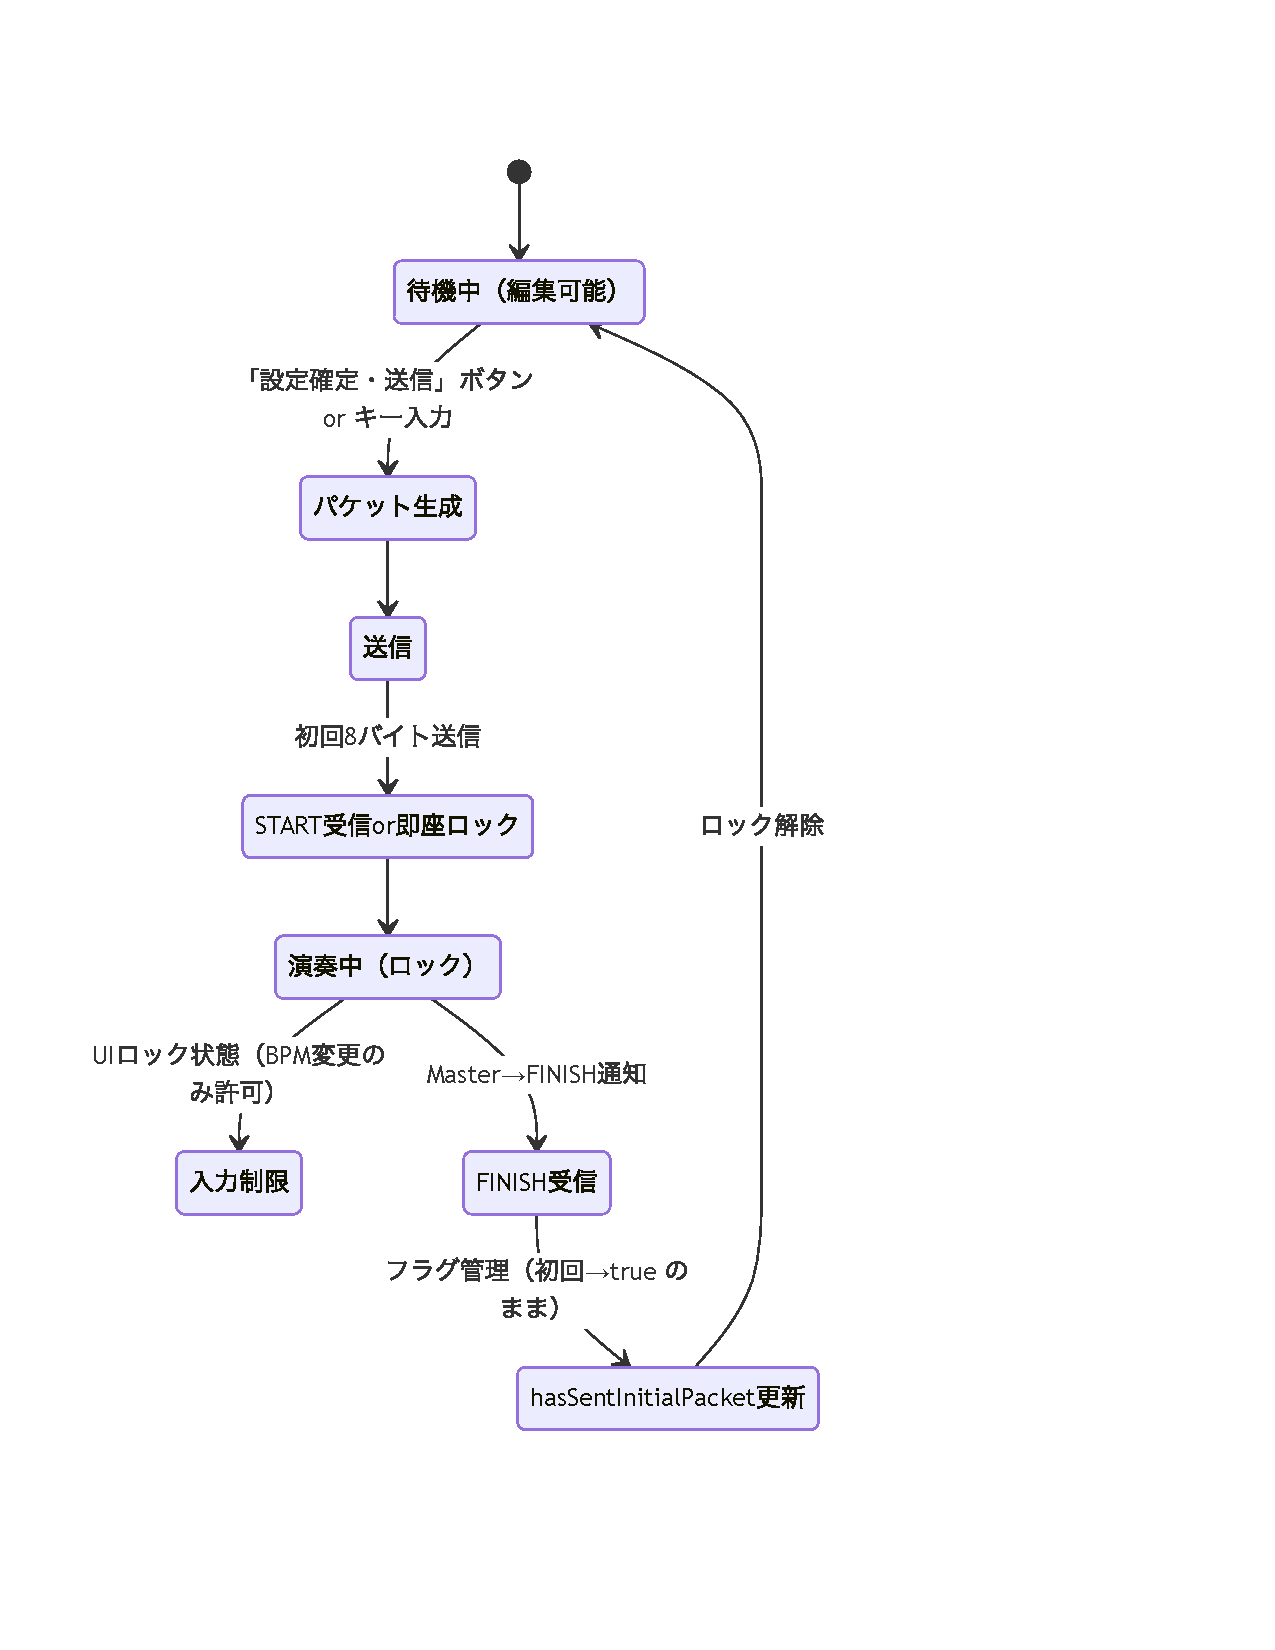
\includegraphics[width=\linewidth]{fig/ProcessingFro.pdf}
    \caption{ProcessingからMasterへの送信の状態遷移図}
    \label{fig:1-6}
\end{wrapfigure}

図\ref{fig:1-6}に，ProcessingからMaster Arduinoへの送信処理における状態遷移を示す．Processing側では，待機中の状態においてBPM，演奏順，オクターブの各設定を受け付け，設定確定・送信操作が行われた時点でパケット生成処理へ遷移する．オクターブは$-1$〜$9$の範囲で入力し，送信時には$00$〜$10$の2桁固定長文字列に変換する．演奏順は楽器1〜3に対応するキー入力をもとに3桁の文字列として保持し，BPMは$30$〜$180$の範囲で3桁固定長の値として扱う．これらの値は\texttt{buildPacket()}によりエンコードされ，Master Arduinoへ送信可能な形式に整形される．
送信処理では，初回送信時と2回目以降で通信内容を切り替える．初回送信では，オクターブ，演奏順，BPMを含む8バイトの初回設定パケットに改行を付加して送信する．一方，2回目以降はBPMのみを3バイトの差分パケットとして送信し，演奏中の通信負荷を抑制する．この分岐は，初回設定済みかどうかを示すフラグによって管理する．
また，Processing側ではMaster Arduinoからの応答を\texttt{serialEvent()}で受信し，状態に応じてUIロック制御を行う．Master Arduinoから\texttt{START}を受信した場合は演奏中のロック状態へ移行し，演奏順およびオクターブの変更を禁止する．\texttt{FINISH}を受信した場合はロックを解除し，再び待機中の編集可能状態へ戻る．この制御により，演奏中の誤操作を防ぎつつ，BPMのみを動的に変更できる入力インタフェースを実現している．

\newpage

\section{担当箇所の詳細設計}
\if0
\subsection{ハードウェア設計}
\subsubsection{回路図とI2Cの原理}
%回路図，部品表（ピン配置含めて），遮光対策（環境光）
図\ref{fig:1-8}に本システムの光同期機能を実現するために必要な回路図，表\ref{tab:1-4}，表\ref{tab:1-5}に本システムで使用する部品表を示す．マスター機1台とスレーブ機4台のArduino Uno R4 WiFiを使用し，主I2Cバスは A4（SDA），A5（SCL）に割り当てられており，USB-Cによる給電およびシリアル通信にも対応している\cite{ref:1-4}．また，受光部にはNJL7502Lのフォトトランジスタを用い，赤外LEDとフォトトランジスタを組み合わせて光信号を検出する．本システムの通信はI2C（Inter-Integrated Circuit）を採用している．I2Cはクロック信号SCLとデータ信号SDAの2本で通信を行う同期式シリアル通信であり，信号線がオープンドレイン構成であるため，HIGHレベルを成立させるには外部プルアップ抵抗が必要である．また，I2Cではcontroller（マスタ）とtarget（スレーブ）の役割を分けて通信を行う．このため，本システムのように複数のArduinoを1つのバスで接続する構成に適している\cite{ref:1-5}．

\begin{figure}[H]
    \centering
    
\includegraphics[width=0.95\textwidth]{fig/HCK01_kairo.pdf}
    \caption{本Arduinoオーケストラの回路図}
    \label{fig:1-8}
\end{figure}

\begin{table}[H]
  \centering
  \caption{部品表：電子部品}
  \label{tab:1-4}
  \small
  \renewcommand{\arraystretch}{1.2}
  \newcolumntype{M}[1]{>{\centering\arraybackslash}m{#1}}
  \newcolumntype{Y}{>{\centering\arraybackslash}X}
  \begin{tabularx}{\textwidth}{|M{3.0cm}|M{2.5cm}|M{1.2cm}|Y|}
    \hline
    \textbf{部品名} & \textbf{型番} & \textbf{個数} & \textbf{用途} 
    \\ \hline
    SDAプルアップ抵抗 & 4.7k$\Omega$ & 1 &
    I2C通信のSDA線をHIGHレベルへ保持する．
     \\ \hline
    SCLプルアップ抵抗 & 4.7k$\Omega$ & 1 &
    I2C通信のSCL線をHIGHレベルへ保持する．
     \\ \hline
    炭素皮膜抵抗 & 220$\Omega$ & 1 &
    LEDの電流制限抵抗として用いる． 
    \\ \hline
    炭素皮膜抵抗 & 10k$\Omega$ & 4 &
    フォトトランジスタ受光回路のプルアップ抵抗として用いる．
     \\ \hline
    フォトトランジスタ & NJL7502L & 4 &
    LED光を受信するための光センサとして用いる．
     \\ \hline
    赤外線LED & ーー & 1 &
    同期信号送信用の光源として用いる． 
    \\ \hline
    遮光装置 & ーー & 1式 &
    外光の影響を抑え，受光値を安定化させる．
     \\ \hline
    ブレッドボード & 165401020E & 必要数 &
    回路の仮組みおよび配線整理に用いる．
     \\ \hline
    ジャンパワイヤ & 165012000E & 1式 &
    各部品間の接続に用いる． 
    \\ \hline
    USBケーブル & ーー & 5 &
    Arduinoの給電およびシリアル通信に用いる．
     \\ \hline
    USBハブ & ーー & 1 &
    複数ArduinoをPCへ同時接続するために用いる．
     \\ \hline
     \end{tabularx}
\end{table}

\begin{table}[H]
  \centering
  \caption{部品表：制御用マイコン}
  \label{tab:1-5}
  \small
  \setlength{\tabcolsep}{4pt}
  \renewcommand{\arraystretch}{1.4}
  \newcolumntype{M}[1]{>{\centering\arraybackslash}m{#1}}
  \newcolumntype{Y}{>{\centering\arraybackslash}X}
  \begin{tabularx}{\textwidth}{|M{1.5cm}|M{1.5cm}|M{1.5cm}|M{4.5cm}|Y|}
    \hline
    \textbf{識別名} &
    \textbf{役割} &
    \textbf{使用ピン} &
    \textbf{接続先} &
    \textbf{主な用途} \\ \hline

    U1 &
    同期制御マスター機 &
    A4(SDA)，A5(SCL)，D2，USB-C &
    SDA/SCLバス，赤外線LED，PC &
    BPM情報をProcessingから受信し，
    I2C通信およびLED光パルスを用いて
    各スレーブ機へ同期信号とBPMを送信する．
    \\ \hline

    U2 &
    ピアノ制御スレーブ機 &
    A4(SDA)，A5(SCL)，D3，USB-C &
    SDA/SCLバス，NJL7502L，PC &
    ピアノ楽譜データの保持，
    光同期検知，Processingへの演奏情報送信を行う．
    \\ \hline

    U3 &
    木琴制御スレーブ機 &
    A4(SDA)，A5(SCL)，D3，USB-C &
    SDA/SCLバス，NJL7502L，PC &
    木琴楽譜データの保持，
    光同期検知，Processingへの演奏情報送信を行う．
    \\ \hline

    U4 &
    フルート制御スレーブ機 &
    A4(SDA)，A5(SCL)，D3，USB-C &
    SDA/SCLバス，NJL7502L，PC &
    フルート楽譜データの保持，
    光同期検知，Processingへの演奏情報送信を行う．
    \\ \hline

    U5 &
    ドラム制御スレーブ機 &
    A4(SDA)，A5(SCL)，D3，USB-C &
    SDA/SCLバス，NJL7502L，PC &
    ドラム楽譜データの保持，
    光同期検知，Processingへの演奏情報送信を行う．
    \\ \hline
  \end{tabularx}
\end{table}

\newpage

\subsubsection{抵抗値の算出}
I2Cのプルアップ抵抗値は，I2Cバスの容量と立ち上がり時間の制約から決定する．I2Cでは信号線がオープンドレイン構成であるため，SDAおよびSCLをHIGHレベルに保つにはプルアップ抵抗が必要である．また，LOW出力時には各デバイスが許容するシンク電流の範囲内に収める必要がある．このとき，プルアップ抵抗値の下限$R_{\mathrm{p(min)}}$は式\ref{eq:1-2}で表される．
\begin{equation}
    R_{\mathrm{p(min)}} = \frac{V_{\mathrm{DD}} - V_{\mathrm{OL(max)}}}{I_{\mathrm{OL}}}
    \label{eq:1-2}
\end{equation}
ここで，$V_{\mathrm{DD}}$は電源電圧，$V_{\mathrm{OL(max)}}$はLOWレベル出力電圧の最大値，$I_{\mathrm{OL}}$はLOWレベル出力時にデバイスに流れ込む引き込み電流（シンク電流）である．式\ref{eq:1-2}に，本システムの設計値である$V_{\mathrm{DD}} = 5.0$ V，$V_{\mathrm{OL(max)}} = 0.4$ V，$I_{\mathrm{OL}} = 3$ mAを代入すると，
\begin{equation}
    R_{\mathrm{p(min)}} = \frac{5.0 - 0.4}{0.003} \approx 1.53 \ \mathrm{k}\Omega
    \label{eq:1-3}
\end{equation}
となる．一方で，抵抗値が大きすぎると信号の立ち上がりが遅くなり，I2Cの仕様を満たせなくなる．立ち上がり時間は，バスの総負荷容量$C_{\mathrm{b}}$とプルアップ抵抗値$R_{\mathrm{p}}$の積に依存する．I2Cの標準モード（Standard-mode）における最大立ち上がり時間$t_{\mathrm{r}}$の規定に基づくと，抵抗値の上限$R_{\mathrm{p(max)}}$は式\ref{eq:1-4}で求められる\cite{ref:1-5}．
\begin{equation}
    R_{\mathrm{p(max)}} = \frac{t_{\mathrm{r}}}{0.8473 \times C_{\mathrm{b}}}
    \label{eq:1-4}
\end{equation}
ここで，$t_{\mathrm{r}}$は最大立ち上がり時間（Standard-modeでは1000 ns），$C_{\mathrm{b}}$はバスの総負荷容量である．本システムのように5台のArduinoを接続し，ジャンパワイヤによる配線を行う場合，$C_{\mathrm{b}}$を約100 pFと仮定すると，$R_{\mathrm{p(max)}}$は約11.8 k$\Omega$となる．したがって，プルアップ抵抗値は$1.53 \ \mathrm{k}\Omega \leq R_{\mathrm{p}} \leq 11.8 \ \mathrm{k}\Omega$の範囲で選定する必要がある．本システムでは，実用上の安定性と汎用性を考慮し，一般的にも広く用いられている4.7 k$\Omega$を採用した．
次に，LEDの電流制限抵抗は，電源電圧，順方向電圧降下，および順方向電流の関係から決定する．電流制限抵抗$R$を算出する式を式\ref{eq:1-5}に示す．
\begin{equation}
    R = \frac{V_{\mathrm{CC}} - V_{\mathrm{F}}}{I_{\mathrm{F}}}
    \label{eq:1-5}
\end{equation}
ここで，$V_{\mathrm{CC}}$は電源電圧，$V_{\mathrm{F}}$はLEDの順方向電圧降下，$I_{\mathrm{F}}$はLEDに流す順方向電流を示す．式\ref{eq:1-5}に，$V_{\mathrm{CC}} = 5.0$ V，$V_{\mathrm{F}} = 2.0$ V，$I_{\mathrm{F}} = 15$ mAを代入すると，
\begin{equation}
    R = \frac{5.0 - 2.0}{0.015} = 200 \ \Omega
    \label{eq:1-6}
\end{equation}
となる．そのため，入手性の高い標準値の中から220 $\Omega$を採用した．
最後に，フォトトランジスタNJL7502Lの受光回路においては，光電流がLEDとの距離，角度，および周囲光の強さなどの環境要因に大きく依存するため，理論式のみで抵抗値を一意に決定することは難しい．このため，本システムでは基準値として10 k$\Omega$を選定し，実装時にArduinoのAnalogReadを用いて受光電圧を測定しながら，実測ベースで逐次調整する方針とした．
\fi

\subsection{ソフトウェア設計}
%全体の処理フローチャート，関数表，変数表，環境光のノイズ除去と閾値の設定について触れる

\subsubsection{全体の処理フロー}
システム全体のフローチャートを図\ref{fig:1-9}に示す．本処理は，Processingの起動時に\texttt{setup()}が実行され，シリアルポートを9600bpsで初期化するところから開始する．接続に成功した場合は\texttt{isSerialConnected}を\texttt{true}に設定し，失敗した場合はシミュレーションモードとして\texttt{isSerialConnected=false}のままUI初期化を完了する．その後は\texttt{draw()}によるメインループに入り，UIの描画とユーザー操作の受付を繰り返す．
ユーザー操作は，BPM変更，演奏順設定，オクターブ変更，送信の4系統に分岐する．BPMは↑／↓キー入力により30〜180の範囲で更新される．演奏順は1〜3キー入力により設定されるが，\texttt{isPlaying=true}の間は変更できず，待機中のみ\texttt{playOrder[]}へ反映される．オクターブもボタンクリックによって-1〜9の範囲で更新されるが，同様に演奏中は操作を無効化する．送信ボタンが押されると\texttt{sendParametersToMaster()}が呼び出され，Master Arduinoへの送信処理へ遷移する．
送信処理では，\texttt{hasSentInitialPacket}の値によって初回送信と2回目以降の送信を切り替える．初回送信では，オクターブ2桁，演奏順3桁，BPM3桁を連結した初回パケットを\texttt{buildPacket()}で生成し，シリアル接続時はMaster Arduinoへ送信する．送信完了後は\texttt{hasSentInitialPacket}を\texttt{true}に更新し，\texttt{isPlaying=true}としてUIをロックする．2回目以降はBPMのみを3桁で送信し，演奏中のテンポ変更に対応する．
また，Master Arduinoからの状態通知は\texttt{serialEvent()}で受信する．\texttt{START}または\texttt{PLAYING}を受信した場合は\texttt{isPlaying=true}を維持してロック状態を継続し，\texttt{FINISH}または\texttt{STOP}を受信した場合は\texttt{isPlaying=false}としてロックを解除する．これにより，演奏中の設定変更を防ぎつつ，演奏終了後は再び設定入力が可能な状態へ戻る．

\begin{figure}[H]
    \centering
    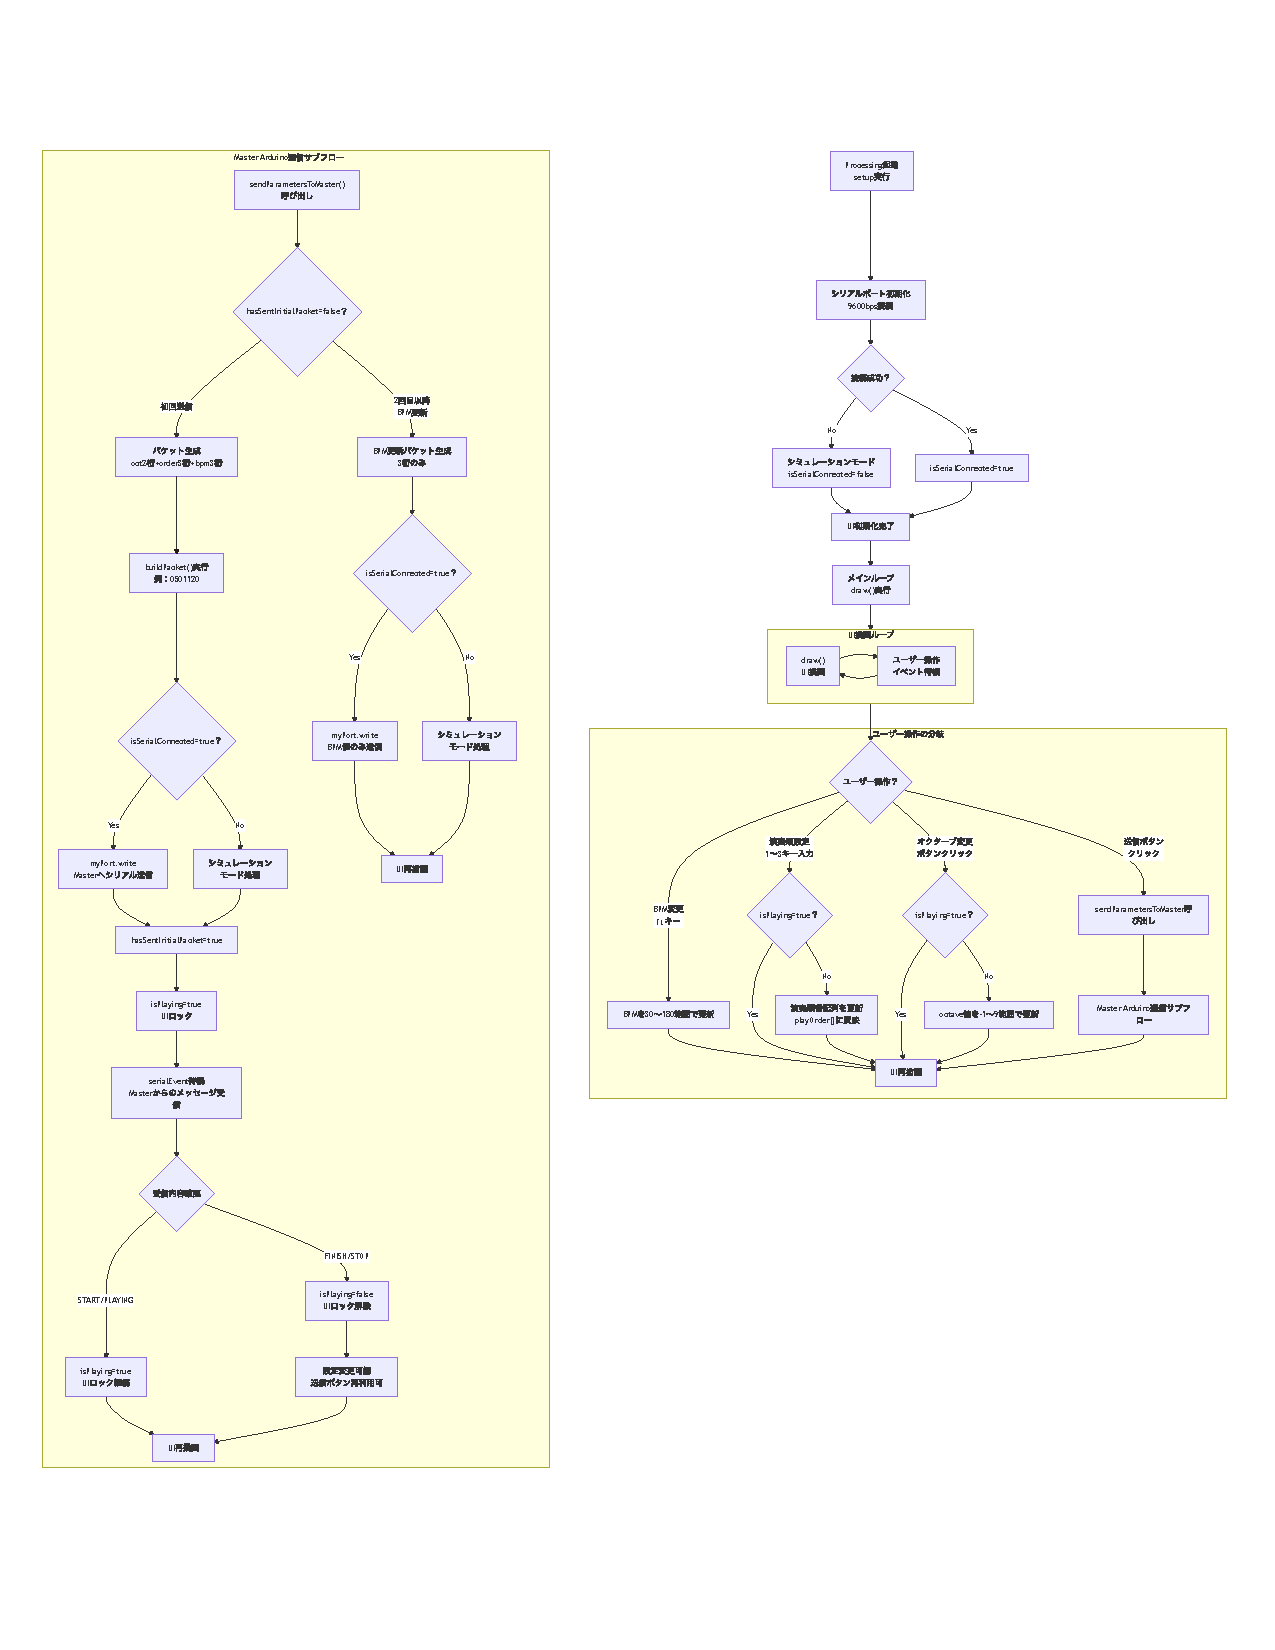
\includegraphics[width=150mm]{fig/zentaiFro2.pdf}
    \caption{UIおよびMaster Arduinoへの送信制御フローチャート}
    \label{fig:1-9}
\end{figure}

\if0
\subsubsection{主要関数表}

表\ref{tab:1-6-1}，表\ref{tab:1-6-2}に示した主要関数について，システムにおける制御の流れに沿ってその役割を述べる．
まず，システムの初期化過程において，Arduino側ではsetupSyncSystemを呼び出し，各ピンの設定，I2Cおよびシリアル通信の初期化，ならびに受光判定に用いる閾値の初期設定を統括して行う．対するProcessing側では，setupSerialChannelsを実行することでArduinoとの通信経路を確立し，受信バッファの構築を行う．
同期信号の送信過程では，マスター機がreceiveBpmFromProcessingを介してProcessingからテンポ情報を取得し，calcBeatIntervalMsによって1拍あたりの時間を算出する．この算出結果に基づき，sendBpmToSlavesによって全Slave機へBPMを一拍前に送信し，sendSyncPulseによってLEDを指定時間点灯させ，同期信号として出力する．
スレーブ機側では，受信したBPMをもとにcalculateDurationMsで音の持続時間を算出し，スロット単位の楽譜管理を行う．受光処理では，sampleAmbientLightを用いて環境光の平均値を取得し，calcThresholdによって適切な余裕幅を加味した閾値を決定する．これにより，detectRisingEdgeを用いた安定した受光判定が可能となり，LEDの点滅を同期基準として抽出する．
演奏制御においては，スレーブ機が光検知の瞬間にactivateCurrentSlotによって現在スロットの楽譜データを有効化し，shiftScoreSlotによって次スロットへ更新する．有効化されたデータはsendNoteDataToProcessingを通じてProcessingへ転送される．Processing側では，シリアル通信の受信をserialEventによってイベント駆動で処理し，parseNotePacketで音高，強さ，長さの各要素へ分解した後，playNoteFromDataへと渡すことで即時的な発音を実現する設計となっている．

\begin{table}[H]
    \centering
    \caption{主要関数表（Arduino側）}
    \label{tab:1-6-1}
    \small
    \renewcommand{\arraystretch}{1.25}
    \newcolumntype{M}[1]{>{\centering\arraybackslash}m{#1}}
    \newcolumntype{Y}{>{\centering\arraybackslash}X}

    \begin{tabularx}{\textwidth}{|M{2.0cm}|M{3.8cm}|M{2.5cm}|Y|}
        \hline
        \textbf{戻り値} & \textbf{関数名} & \textbf{引数} & \textbf{役割} \\ \hline

        \multicolumn{4}{|c|}{\textbf{Arduino（Master）}} \\ \hline
        void & setup & なし & 初期化の起点であり，ピン設定，通信設定，閾値初期化をまとめて実行する． \\ \hline
        void & loop & なし & 主処理を繰り返し実行し，MasterまたはSlaveの役割に応じて分岐する． \\ \hline
        void & setupSyncSystem & なし & ピン設定，I2C初期化，シリアル初期化，閾値用の初期値設定をまとめて行う． \\ \hline
        float & receiveBpmFromProcessing & なし & Processingから送られたBPMを受信し，有効範囲を確認したうえで返す． \\ \hline
        unsigned long & calcBeatIntervalMs & bpm & BPMから1拍あたりの時間を算出する．$T=60000/\mathrm{BPM}$ に対応する． \\ \hline
        void & sendBpmToSlaves & bpm & 受信したBPMを全Slave機へ一拍前に送信する． \\ \hline
        void & sendSyncPulse & pulseWidthMs & マスター機のLEDを指定時間だけ点灯させ，同期信号として出力する． \\ \hline

        \multicolumn{4}{|c|}{\textbf{Arduino（Slave）}} \\ \hline
        void & setup & なし & 初期化の起点であり，ピン設定，通信設定，閾値初期化をまとめて実行する． \\ \hline
        void & loop & なし & 主処理を繰り返し実行し，受光判定と楽譜スロット更新を行う． \\ \hline
        void & setupSyncSystem & なし & ピン設定，I2C初期化，シリアル初期化，閾値用の初期値設定をまとめて行う． \\ \hline
        float & receiveBpmFromMaster & なし & Masterから送られたBPMを受信し，有効範囲を確認したうえで返す． \\ \hline
        uint16\_t & sampleAmbientLight & sampleCount & 環境光を複数回取得し，平均値を求める． \\ \hline
        uint16\_t & calcThreshold & ambientAverage, margin & 環境光平均値に余裕幅を加えて受光判定の閾値を算出する． \\ \hline
        bool & detectRisingEdge & sensorValue, thresholdValue & 受光値が閾値を上回った瞬間を検出し，LED点滅を認識する． \\ \hline
        unsigned long & calculateDurationMs & durationSlots, beatIntervalMs & 8分音符を1スロットとした楽譜管理に基づき，音の持続時間を算出する． \\ \hline
        NoteData & activateCurrentSlot & scoreSlots, slotIndex & 現在スロットの楽譜データを有効化し，発音対象を返す． \\ \hline
        void & shiftScoreSlot & なし & 現在スロットを次へ進め，次回の受光に備える． \\ \hline
        void & sendNoteDataToProcessing & noteData & 受光検知後に，保持していた音符データをProcessingへ送信する． \\ \hline
    \end{tabularx}
\end{table}

\begin{table}[H]
    \centering
    \caption{主要関数表（Processing側）}
    \label{tab:1-6-2}
    \small
    \renewcommand{\arraystretch}{1.25}
    \newcolumntype{M}[1]{>{\centering\arraybackslash}m{#1}}
    \newcolumntype{Y}{>{\centering\arraybackslash}X}

    \begin{tabularx}{\textwidth}{|M{2.0cm}|M{3.8cm}|M{2.5cm}|Y|}
        \hline
        \textbf{戻り値} & \textbf{関数名} & \textbf{引数} & \textbf{役割} \\ \hline
        void & setupSerialChannels & なし & Arduinoとの通信に使うシリアルポートを開き，受信バッファを設定する． \\ \hline
        void & sendBpmToMaster & bpm & UIで入力されたBPMをマスター機へ送信する． \\ \hline
        void & serialEvent & port & データ到着時に呼び出され，スレーブ機からの音符データを受信する． \\ \hline
        NoteData & parseNotePacket & packet & 受信した文字列またはバイト列を解析し，音高，強さ，長さに分解する． \\ \hline
        void & playNoteFromData & noteData & 受信した音符データに基づいて音色を生成し，発音する． \\ \hline
    \end{tabularx}
\end{table}

\subsubsection{主要変数および定数}

表\ref{tab:1-7}に示した主要変数および定数について，各パラメータがシステム動作に果たす役割を述べる．
同期制御を司るパラメータとして，初期テンポを規定するdefaultBpm，Master側で算出された1拍あたりの待機時間を保持するbeatIntervalMs，および同期信号のパルス幅を固定するledPulseWidthMsが動作の基準となる．Master側では受信したBPMをreceivedBpmに保持し，全Slave機への送信準備状態を管理する．
Slave側では，受信したBPMをもとにbeatIntervalMsからslotDurationMsを算出し，8分音符を1スロットとした楽譜管理を行う．scoreSlotsは楽譜配列そのものであり，slotIndexが現在位置を示す．currentNoteは現在スロットで有効化された音符データ，currentDurationSlotsはその長さをスロット数で保持する．受光判定に関連する変数群では，環境光の平均化処理に用いるサンプル数ambientSampleCountと，その測定結果であるambientAverageが基礎となる．これに判定の余裕幅であるthresholdMarginを加算することで，最終的な判定基準となる閾値thresholdValueが決定される．現在のセンサー測定値はsensorValueに格納され，立ち上がり検知の結果はフラグlightDetectedによって動的に管理される．
Processing側の制御においては，ユーザーインターフェースから入力されたテンポ情報を保持するbpmInputや，各機体との通信を確立するためのmasterPortおよびslavePortsが中核となる．受信したデータはrxBufferにおいて一時的に保存され，受信状態を示すreceivingFlagによる制御を経て，最終的に解析済みの音符データとしてreceivedNoteに格納される構成を採っている．

\begin{table}[H]
    \centering
    \caption{主要変数および定数表}
    \label{tab:1-7}
    \small
    \renewcommand{\arraystretch}{1.25}
    \newcolumntype{M}[1]{>{\centering\arraybackslash}m{#1}}
    \newcolumntype{Y}{>{\centering\arraybackslash}X}

    \begin{tabularx}{\textwidth}{|M{2.4cm}|M{3.2cm}|M{1.8cm}|Y|}
        \hline
        \textbf{型} & \textbf{変数名} & \textbf{初期値} & \textbf{役割} \\ \hline

        \multicolumn{4}{|c|}{\textbf{Arduino（Master）}} \\ \hline
        \textbf{型} & \textbf{変数名} & \textbf{初期値} & \textbf{役割} \\ \hline
        const float & defaultBpm & 120.0 & 初期BPMとして使用する． \\ \hline
        float & receivedBpm & 120.0 & Processingから受信したBPMを保持する． \\ \hline
        unsigned long & beatIntervalMs & 500 & 1拍あたりの点滅間隔を保持する． \\ \hline
        const unsigned int & ledPulseWidthMs & 10 & LED点滅時間を10 msに固定する． \\ \hline

        \multicolumn{4}{|c|}{\textbf{Arduino（Slave）}} \\ \hline
        \textbf{型} & \textbf{変数名} & \textbf{初期値} & \textbf{役割} \\ \hline
        const uint8\_t & ambientSampleCount & 32 & 環境光平均化のためのサンプル数を定める． \\ \hline
        uint16\_t & ambientAverage & 0 & 起動時に取得した環境光の平均値を保持する． \\ \hline
        uint16\_t & thresholdMargin & 20 & 閾値に加える余裕幅を保持する． \\ \hline
        uint16\_t & thresholdValue & 0 & 受光判定の閾値を保持する． \\ \hline
        uint16\_t & sensorValue & 0 & 現在の受光値を保持する． \\ \hline
        bool & lightDetected & false & LED点滅を検知したかどうかを管理する． \\ \hline
        float & receivedBpm & 120.0 & Masterから受信したBPMを保持する． \\ \hline
        unsigned long & beatIntervalMs & 500 & 受信BPMから算出した1拍時間を保持する． \\ \hline
        unsigned long & slotDurationMs & 250 & 1スロットあたりの持続時間を保持する． \\ \hline
        NoteData[] & scoreSlots & 初期楽譜 & 8分音符を1スロットとした楽譜配列を保持する． \\ \hline
        uint8\_t & slotIndex & 0 & 現在の楽譜スロット位置を示す． \\ \hline
        NoteData & currentNote & pitch=0, velocity=0, durationSlots=1 & 現在スロットで有効化された音符データを保持する． \\ \hline
        uint8\_t & currentDurationSlots & 1 & 現在音符の持続時間をスロット数で保持する． \\ \hline

        \multicolumn{4}{|c|}{\textbf{Processing}} \\ \hline
        \textbf{型} & \textbf{変数名} & \textbf{初期値} & \textbf{役割} \\ \hline
        float & bpmInput & 120.0 & UIで入力されたBPMを保持する． \\ \hline
        Serial & masterPort & 未接続 & マスター機との通信用ポートを保持する． \\ \hline
        Serial[] & slavePorts & 未接続 & スレーブ機との通信用ポート群を保持する． \\ \hline
        String & rxBuffer & ``'' & 受信した文字列データを一時保持する． \\ \hline
        boolean & receivingFlag & false & 受信処理中かどうかを管理する． \\ \hline
        NoteData & receivedNote & pitch=0, velocity=0, durationSlots=1 & 受信後の音符データを保持する． \\ \hline
    \end{tabularx}
\end{table}

\newpage

\subsubsection{閾値の検討および楽譜配列のスロット更新処理}
本システムでは，受光値をanalogReadで取得し，環境光の平均値を基準として閾値を設定する．この方式により，窓からの自然光や天井灯の影響を受けても，相対的な変化としてLED点滅を判定できる．ただし，本節では遮蔽物がある場合のBPM固定演奏は扱わず，例外処理として別節で説明する．
\begin{lstlisting}[language=C++,caption={受光閾値の算出とスロット更新処理},label={code:threshold}]
const uint8_t sensorPin = D3;
const uint16_t ambientSampleCount = 32;
const uint16_t thresholdMargin = 20;

uint16_t ambientAverage = 0;
uint16_t thresholdValue = 0;
uint16_t sensorValue = 0;
bool lightDetected = false;

float receivedBpm = 120.0;
unsigned long beatIntervalMs = 500;
unsigned long slotDurationMs = 250;

uint8_t slotIndex = 0;
uint8_t currentDurationSlots = 1;
NoteData currentNote;

NoteData scoreSlots[] = { ... };  \% 実際の楽譜データ
uint8_t currentDurationSlots = 1;

void setup() {
  Serial.begin(115200);
  pinMode(sensorPin, INPUT);

  ambientAverage = sampleAmbientLight(ambientSampleCount);
  thresholdValue = calcThreshold(ambientAverage, thresholdMargin);
}

uint16_t sampleAmbientLight(uint16_t sampleCount) {
  uint32_t sum = 0;
  for (uint16_t i = 0; i < sampleCount; i++) {
    sum += analogRead(sensorPin);
    delay(5);
  }
  return sum / sampleCount;
}

uint16_t calcThreshold(uint16_t ambientAvg, uint16_t margin) {
  return ambientAvg + margin;
}

bool detectRisingEdge(uint16_t value, uint16_t threshold) {
  static bool previousAbove = false;
  bool currentAbove = (value >= threshold);
  bool risingEdge = (!previousAbove && currentAbove);
  previousAbove = currentAbove;
  return risingEdge;
}

unsigned long calculateDurationMs(uint8_t durationSlots, unsigned long beatMs) {
  unsigned long slotMs = beatMs / 2;
  return (unsigned long)durationSlots * slotMs;
}

NoteData activateCurrentSlot(NoteData scoreSlots[], uint8_t index) {
  return scoreSlots[index];
}

void shiftScoreSlot() {
  slotIndex++;
}

void loop() {
  sensorValue = analogRead(sensorPin);
  lightDetected = detectRisingEdge(sensorValue, thresholdValue);

  if (lightDetected) {
    currentNote = activateCurrentSlot(scoreSlots, slotIndex);
    slotDurationMs = calculateDurationMs(currentNote.durationSlots, beatIntervalMs);
    sendNoteDataToProcessing(currentNote);
    shiftScoreSlot();
  }
}
\end{lstlisting}
1行目から4行目では，受光入力ピン，サンプル数，余裕幅を定数として定義している．6行目から14行目では，平均値，閾値，現在値，受光フラグ，BPM，1拍時間，スロット時間，現在スロット位置，現在音符を保持する変数を定義している．16行目から23行目のsetupでは，シリアル通信の開始，ピン設定，環境光平均値の取得，閾値計算を順に実行している．25行目から32行目のsampleAmbientLightでは，複数回のanalogReadを平均して環境光の影響をならしている．34行目から36行目のcalcThresholdでは，平均値に余裕幅を加えて閾値を決めている．38行目から44行目のdetectRisingEdgeでは，前回値と現在値を比較し，閾値を下から上へ超えた瞬間だけを検知している．46行目から49行目のcalculateDurationMsでは，8分音符を1スロットとした持続時間を算出している．51行目から53行目のactivateCurrentSlotでは，現在の楽譜スロットを取り出して有効化している．55行目から57行目のshiftScoreSlotでは，受光後に次のスロットへ進めている．59行目から66行目のloopでは，受光値を読み取り，立ち上がり検知が成立したときに現在スロットを有効化し，持続時間を計算したうえでProcessingへ通知している．


\begin{thebibliography}{9}
%\bibitem{ref:1-1}難波精一郎（$2012$）「時間，音そして音楽─実験心理学的観点から─」『日本音楽知覚認知学会』第$18$巻第$1\&2$号
\bibitem{ref:1-2} 宮坂泰弘，近藤康太郎，森道昭，神門正城，桐山博光（$2024$）「光同期光パラメトリックチャープパルス増幅法励起のための高安定サブナノ秒Nd:YAGレーザー」『レーザー研究』第$52$巻第$2$号，p.79--83．
\bibitem{ref:1-3}新日本無線（$2013$）「照度センサNJL7502L」\\
\url{https://akizukidenshi.com/goodsaffix/NJL7502L_J.pdf}
\bibitem{ref:1-4}Arduino（$2023$）「Arduino Uno R4 WiFi aProduct Reference Manual」\\
\url{https://akizukidenshi.com/goodsaffix/ABX00087.pdf}
\bibitem{ref:1-5} NXP Semiconductors（$2021$）「UM10204 I2C-bus specification and user manual Rev. 7.0」\\
\url{https://www.nxp.com/docs/en/user-guide/UM10204.pdf}

\end{thebibliography}
\fi
\end{document}